% !TeX spellcheck = en_GB
\documentclass[abstract,toc,los,english,10pt,glossaries]{jluthesis}

\usepackage{pdfpages}
\newacronym{eas}{EAS}{Extensive Air Showers}
\newacronym{uhecr}{UHECR}{Ultra High Energy Cosmic Radiation}
\newacronym{sipm}{SiPM}{Silicon Photomultiplier}
\newacronym{adc}{ADC}{Analog Digital Converter}
\newacronym{enu}{ENU}{East, North Up}
\newacronym{com}{COM}{center of mass}
\newacronym{csda}{CSDA}{continuous-slowing-down approximation}
\newacronym{gzkl}{GZK-Limit}{Greisen–Zatsepin–Kuzmin limit}
\newglossaryentry{hadron} {name=hadron, description={subatomic particle affected by the strong interaction}}
\newglossaryentry{nucleus} {name=nucleus, plural=nuclei, description={Center of an atom}}
\bibliography{data/thesis.bib}

\topic{Real-time data analysis of distributed muon detector network for cosmic shower detection and reconstruction}
\title[Bachelor Thesis]{Bachelor Thesis}
\author[Daniel Treffenstädt]{Daniel J.S. Treffenstädt}
\matnr{6067797}
\reviewer{Prof. Dr. Kai-Thomas Brinkmann\\Prof. Dr. Sören Lange}
\supervisor{Dr. Hans-Georg Zaunick}




\begin{document}
\makebeginning{
	Extensive Air Showers produced by ultra high energy cosmic radiation is still an active area of research. Due to the low number of such events collecting statistics is not a simple task. There are many approaches to collecting enough data about these air showers. One such approach is the usage of a distributed network of low-cost particle detectors which can be operated by persons outside the university environment.
	
	In this thesis, a method is developed to perform real-time analysis for a network of low-cost plastic scintillator detectors. This network consists of small scintillator detectors with silicon Photomultiplier units which are attached to a Raspberry-Pi computer. Those detection units are located throughout Germany and send their data to a server where it is continuously monitored for coincidences.
	
	An approach to reconstructing the possible incident direction of the primary particle as well as an approximation for plausible energies is presented.
}
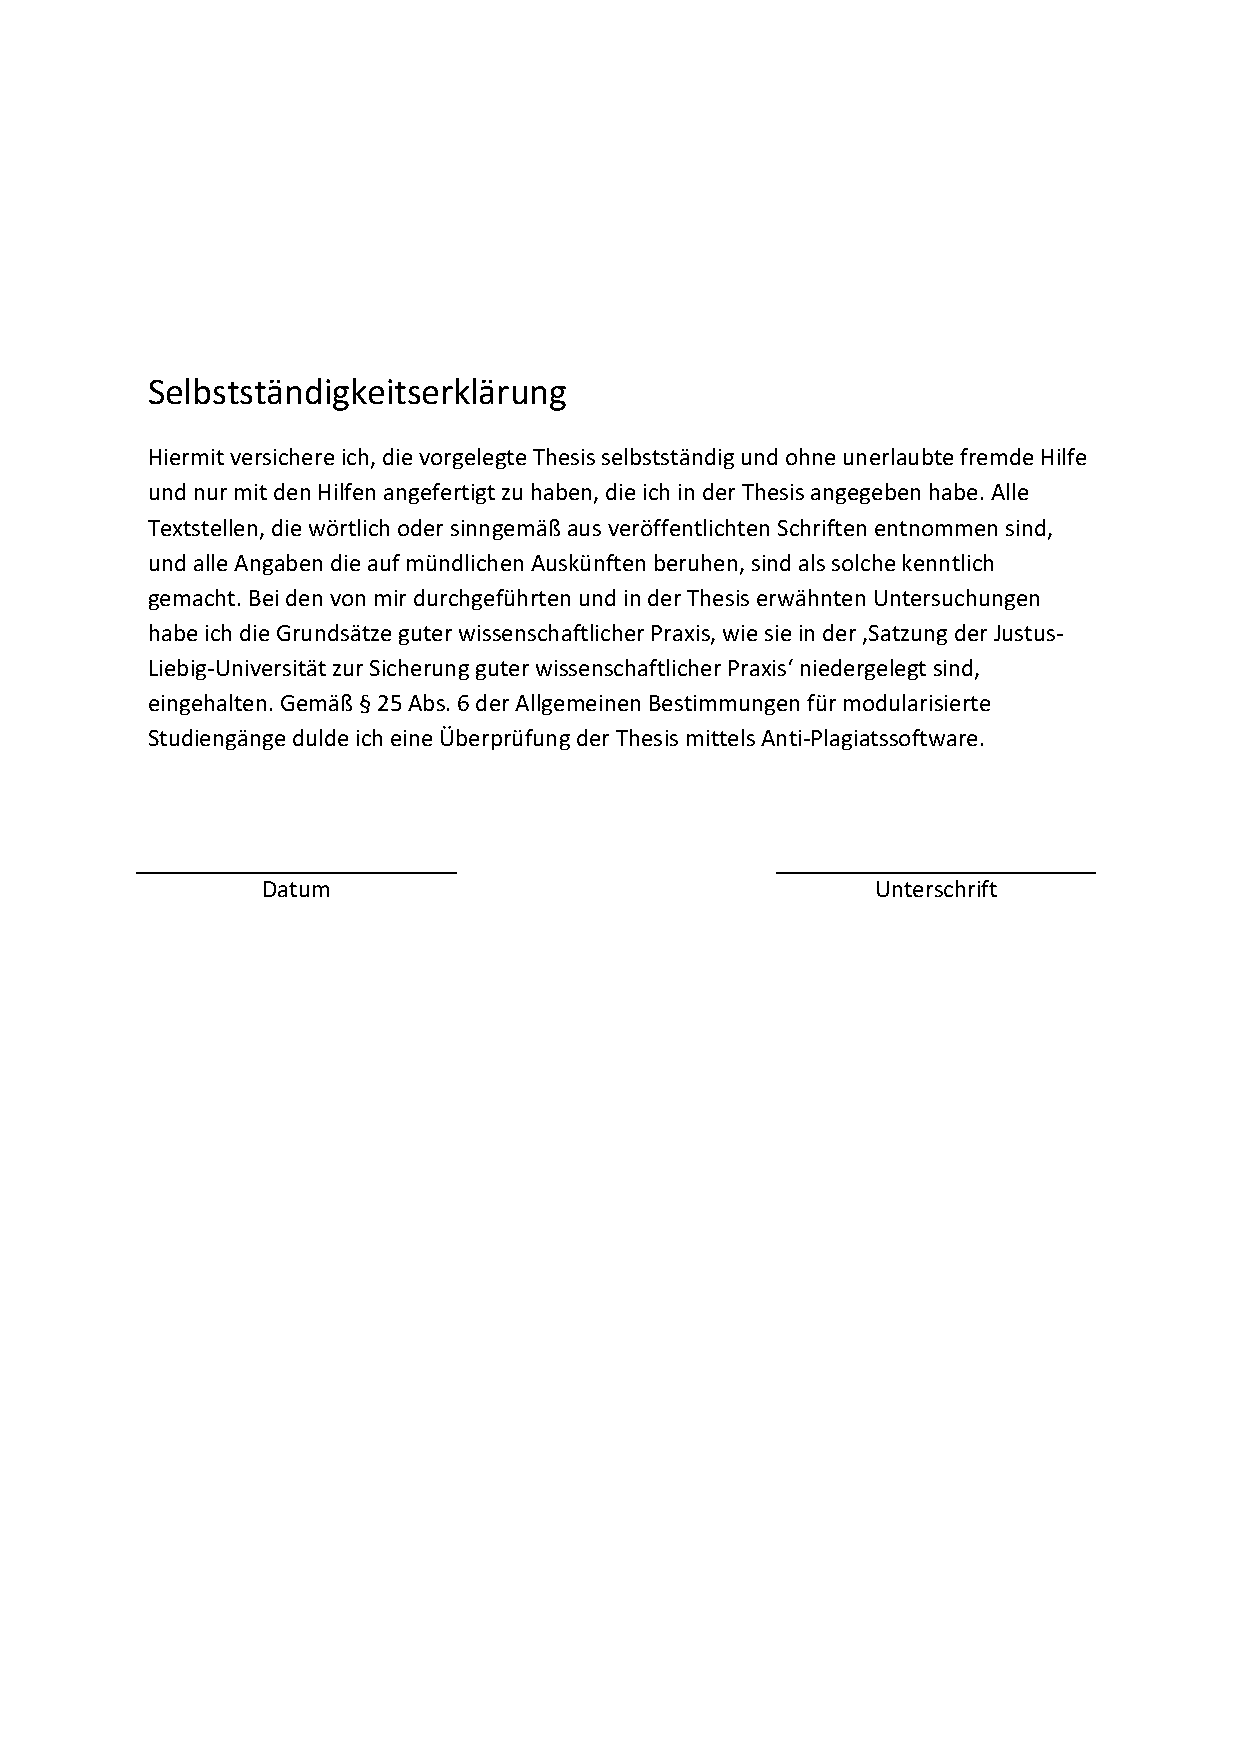
\includepdf[noautoscale=true, width=\paperwidth]{data/selbststaendigkeit.pdf}


\section{Introduction}
\subsection{Cosmic Radiation}
\acrfull{uhecr} is cosmic radiation with energy in the range of $10^{18}$\,eV to $10^{20}$\,eV.\footnote{The energy unit eV(Electron-Volt) describes the kinetic energy a unit charge holds after being accelerated through an electric field for 1V. It is equivalent to $1.602176634\cdot10^{-19}\,\text{J}$.}
Cosmic radiation has been discovered in 1912 by Viktor Hess by performing measurements with three electrometers in a balloon flight. He measured the energy flux in the atmosphere and showed that it increased with altitude. This is explained by secondary particles which are produced through the interaction of primary cosmic radiation with the atmosphere. The cosmic radiation is produced by many different sources, one of which is our sun. The sun however only produces cosmic radiation up to a few hundred MeV of energy through coronal mass ejections and other processes and so is not contributing to \acrshort{uhecr}. Higher energy sources include other stars, supernovae and also black holes. \\
\begin{figure}[ht!]
	\centering
	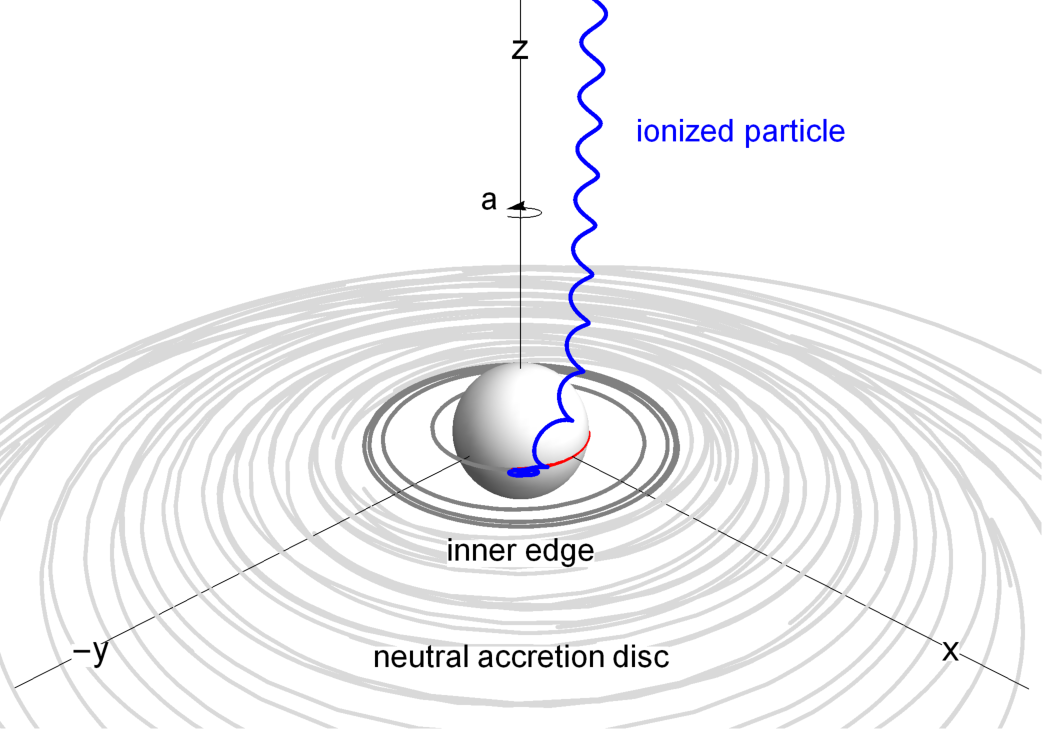
\includegraphics[width=0.5\linewidth]{data/uhecr-sm-bh}
	\caption{Trajectory of neutral particle around supermassive black hole \cite{Tursunov_2020}}
	\label{fig:uhecr-sm-bh}
\end{figure}\\
The production mechanisms for \acrshort{uhecr} are unknown and an area of active research, though some sources have been speculated. One such proposed mechanism is a spinning supermassive hole with a neutral particle in its accretion disk. The Orbit of this particle decays until it is close enough to the black hole so that the effective electric charge dominates and ionises the particle which causes a large acceleration\cite{Tursunov_2020}. The trajectory of the particle is shown in figure \ref{fig:uhecr-sm-bh}.\\
\begin{figure}[ht!]
	\centering
	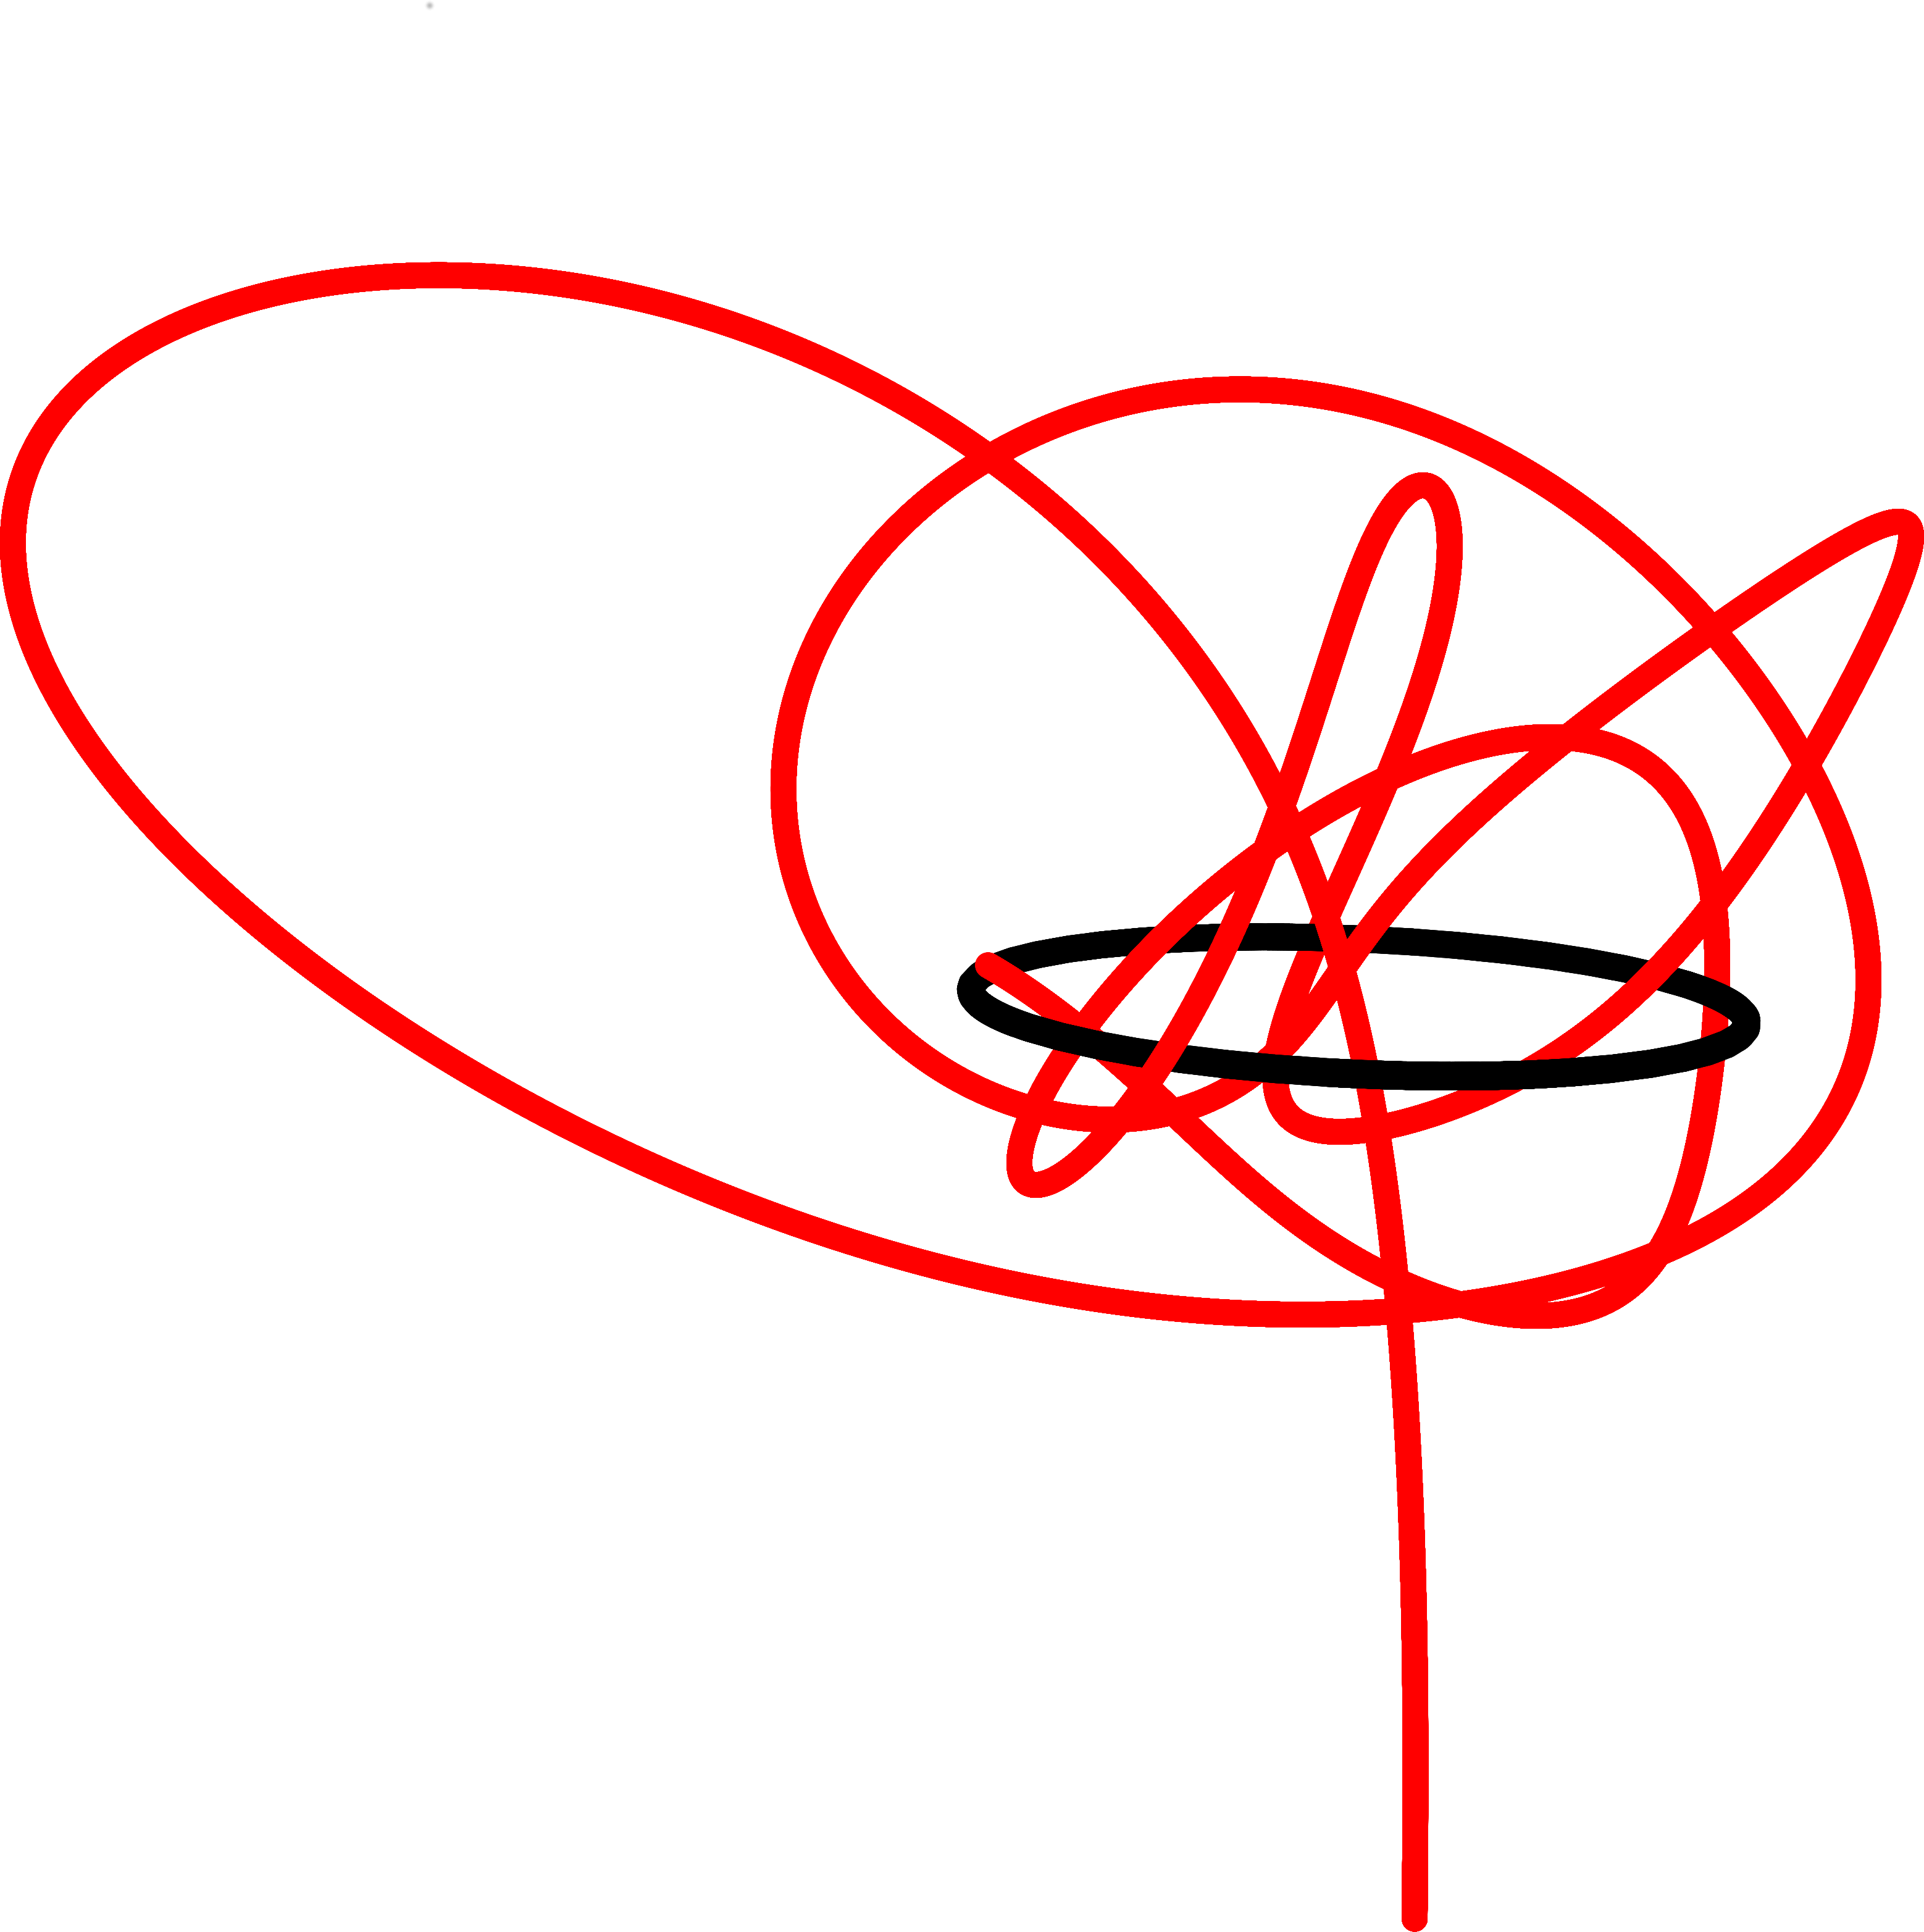
\includegraphics[width=0.4\linewidth]{data/trajectory-binary-bh}
	\caption{Possible trajectory of UHECR in Binary Black hole system \cite{Zhang2020}}
	\label{fig:trajectory-binary-bh}
\end{figure} \\
Already high energy particles can be accelerated to the ultra high energy regime. One possible acceleration mechanism relies on a pair of binary black holes which move at relativistic speeds. In such a scenario the particle can experience a series of gravitational slingshots \cite{Zhang2020} around the binary system and finally be accelerated so much it reaches the necessary energy region to be classified as an \acrshort{uhecr}. One possible trajectory of a particle that lead to an \acrshort{uhecr} which has been simulated is shown in figure \ref{fig:trajectory-binary-bh}. \\
\begin{figure}[ht!]
	\centering
	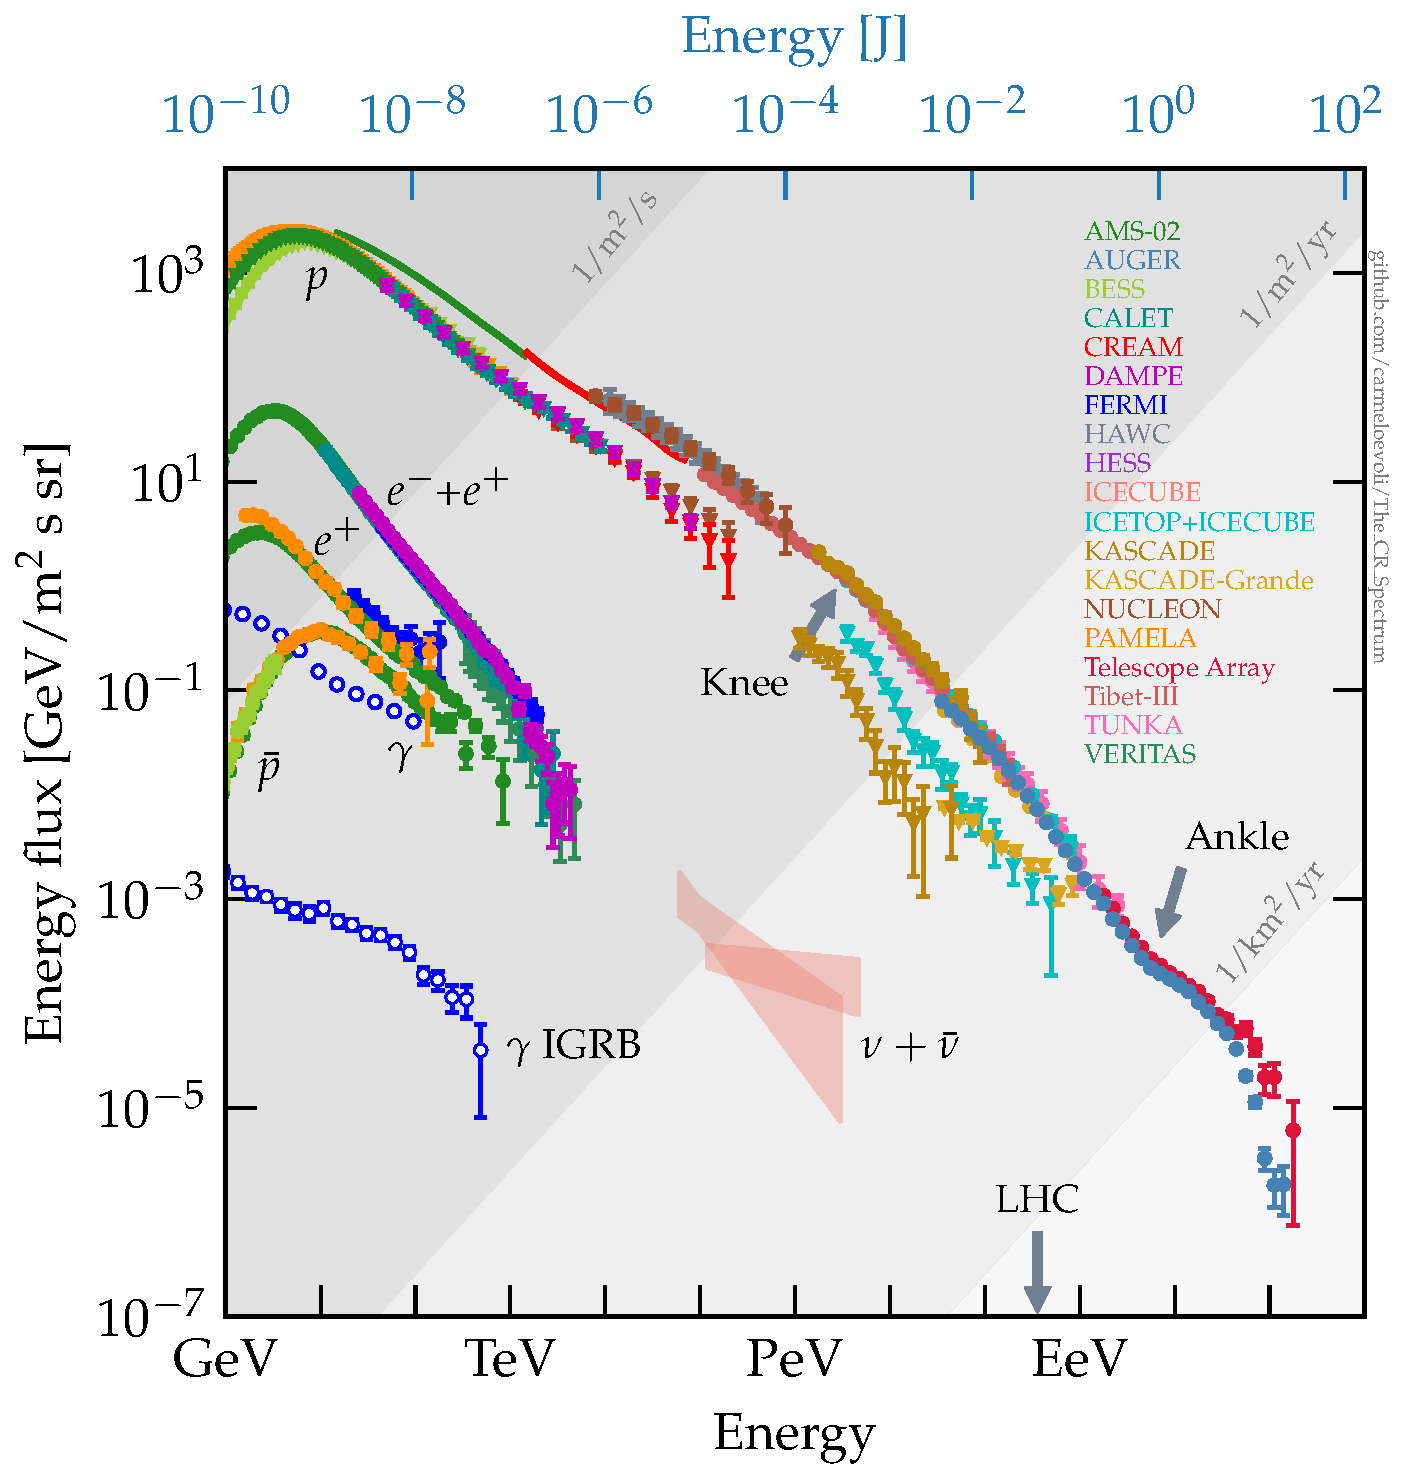
\includegraphics[width=0.75\linewidth]{data/cr_spectrum}
	\caption{Spectrum of cosmic radiation \cite{evoli_carmelo_2020_4396125}}
	\label{fig:cr_spectrum}
\end{figure} \\
The spectrum of this cosmic radiation is shown in figure \ref{fig:cr_spectrum}. There, measurements from different experiments are shown. The y axis shows the energy flux of cosmic rays in units of energy per second per square meter per solid angle $\frac{\text{GeV}}{\text{m}^2\cdot\text{s}\cdot\text{sr}}$. The x axis shows the primary energy of the cosmic rays, for comparison the upper axis shows the energy in units of Joule, the lower axis shows it in units of electron-Volt. Notable here is the much higher number of protons as compared to all other particles by two orders of magnitude. This allows one to make the reasonable assumption that most cosmic rays are protons. Prominent features of the proton spectrum are two anomalies labeled as Knee and Ankle. \\
One interesting observation is that the proton spectrum does not have a solid cutoff at $5\cdot10^{19}$\,eV of energy, rather it extends beyond it. This value is significant because it is calculated to be the \acrfull{gzkl}\cite{2021APh...12602526B}. This limit stems from high energy protons interacting with the microwave background radiation and being lifted into an excited state.
\begin{equation}\label{eq:gzkl}
	\begin{aligned}
		\gamma + p &\rightarrow \Delta^+ &\rightarrow p + \pi^0 \\
		\gamma + p &\rightarrow \Delta^+ &\rightarrow n + \pi^+
	\end{aligned}
\end{equation}
Equation \ref{eq:gzkl} descibes the possible interaction between the microwave background photons and protons. In both cases, the proton gets excited to a $\Delta^+$ resonance state, which can decay to a hadron and a pi meson. One possible decay product is a proton and a $\pi^0$, the other one a neutron and a $\pi^+$. In this process, the proton loses roughly $20\,\%$ of its energy, since the energy prior to the interaction gets transferred to both resulting particles according to their relative masses. Should the proton then remain above the limit, the same interaction can take place again. It is unlikely that any proton at these energies can travel more than $100\,\cdot10^6\,\text{ly}$ without undergoing this interaction. Since most particles above the ankle in the proton specturm shown in figure \ref{fig:cr_spectrum} are of extragalactic origin, this means that virtually all protons with these high energies must have undergone this interaction, dropping them below the \acrshort{gzkl}.
The violation of this limit could be explained with a proposition by the Pierre Auger Observatory that most \acrshort{uhecr} are in fact heavier nuclei than single protons \cite{thepierreaugercollaboration2017inferences}.

\subsection{Cosmic Air Showers}\label{subsec:airshowers}
When a cosmic ray hits the atmosphere, it interacts with the nucleons of the different molecules in air. Due to the relative abundance, it is most likely that the first interaction takes place between the primary particle and a Neutrogen nucleus. This causes interactions described by Quantum Chromo dynamics which is beyond the scope of this thesis. This interaction leaves nucelar fragments and $\pi$ mesons behind which can then interact with other air molecules again or - in the case of pions - decay. This creates a cascade of particles which continue along the trajectory towards the surface of earth. A picture of an air shower produced by a primary proton is shown in figure \ref{fig:proton-shower}. This image is produced at the KIT with the simulation toolkit CORSIKA.
\begin{figure}[ht!]
	\centering
	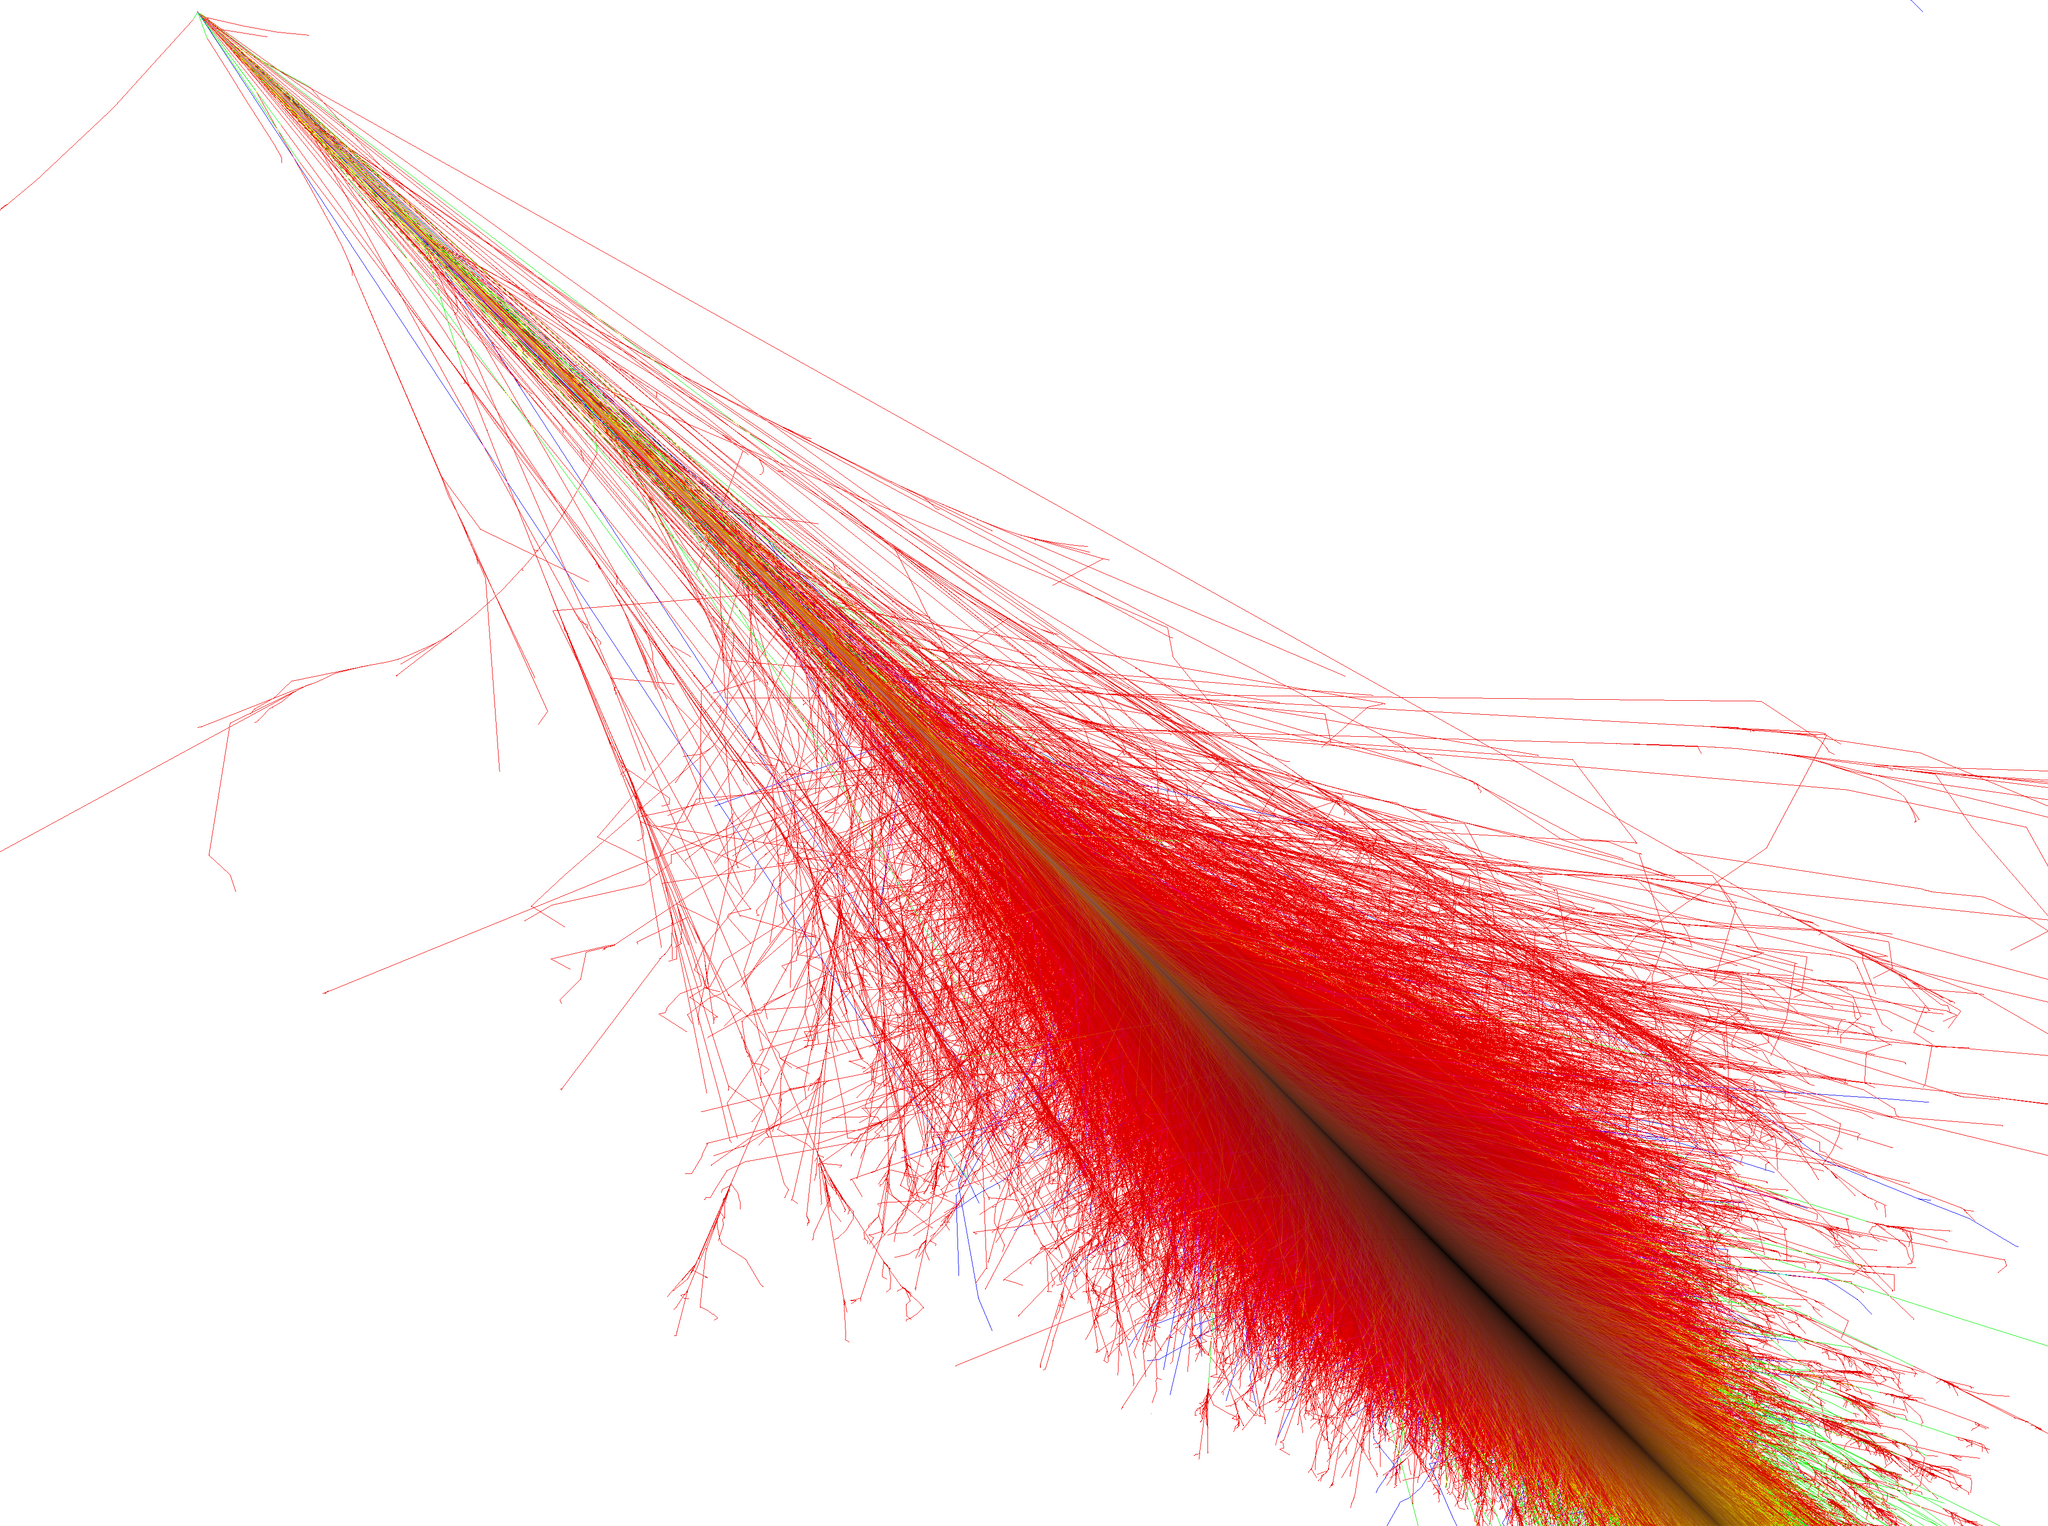
\includegraphics[width=0.8\linewidth]{data/shower-45}
	\caption{Proton Air Shower \cite{corsika-images}}
	\label{fig:proton-shower}
\end{figure} \\

The secondary particles can be divided into three different components, they are shown in figure \ref{fig:shower-components}.
As seen in this figure, neutral Pions $\pi^0$ can decay to two photons $\gamma$ or an electron positron pair and a photon. The decay cross section for the two gamma production is much higher than that of the $e^\pm + \gamma$ production though, resulting in probabilities of roughly $99$ and $1\,\%$. 
\begin{equation}
	\begin{aligned}
		\pi^0 &\rightarrow 2\gamma \\
		\pi^0 &\rightarrow e^+ + e^- + \gamma \\
	\end{aligned}
\end{equation}
The produced photons can then undergo pair production through which a lepton - anti lepton pair is produced. For this to occur, the photon needs to have an energy higher than twice the rest mass of the lepton. In the case of an electron positron pair, the rest energy is $511\,\text{keV}$ resulting in a minimum photon energy of $1022\,\text{keV}$. Any energy above this limit gets distributed evenly across both resulting particles as kinetic energy. In the \acrfull{com} system due to conservation of impulse, the pair travels in opposite directions to each other in a 90 degree angle to the original photon. In the laboratory system however, the resulting particles continue along the original trajectory.
\todo{sources for decay probabilities}
Should the photon not have enough energy to produce a pair, it can be absorbed in an atom by raising the energy level of an electron in the shell or loose energy through compton scattering.\\
In the case of a charged pion $\pi^\pm$, The most likly decay with a probability of $99.9\,\%$ is to a muon $\mu^\pm$ and a muon-neutrino $\nu_\mu$. The interaction is shown in equation \ref{eq:piondecay}.
\begin{equation}\label{eq:piondecay}
	\begin{aligned}
		\pi^+ &\rightarrow \mu^+ + \nu_\mu \\
		\pi^- &\rightarrow \mu^- + \bar{\nu}_\mu
	\end{aligned}
\end{equation}
\begin{figure}[ht!]
	\centering
	\begin{tikzpicture}
		\draw[->] (0,0.5) node[above] {primary particle} -- ++(0,-1.5) coordinate(primary);
		\draw[->] (primary) -- ++(-175:1.5) node[above] {$\pi^0$} -- ++(-175:2) coordinate (pi0);
		\draw[->] (primary) -- ++(-105:1) node[left] {$\pi^\pm$} -- ++(-105:1.5) coordinate (pipm);
		\draw[->] (primary) -- ++(-35:1) -- ++ (-35:2) coordinate (zn);
		
		\draw[->] (pi0) -- ++(-160:1) coordinate(gamma) node[above right] {$\gamma$};
		\draw[->] (pi0) -- ++(-130:1) node[below right] {$\gamma$};
		\draw[->] (gamma) -- ++(-165:1) node[above] {$e^\pm$};
		\draw[->] (gamma) -- ++(-155:1) node[below] {$e^\mp$};
		
		\draw[->] (pipm) -- ++(-110:1) node[left] {$\mu^\pm$};
		
		\draw[->] (zn) -- ++(-10:1) node[above] {p};
		\draw[->] (zn) -- ++(-30:1) node[below] {n};
		
		\draw[thin, dashed] (-2,0) -- ++(0,-5) ++ (-0.5,0) node[left] {Electromagnetic};
		\draw[thin, dashed] (2,0) -- ++(0,-5) ++(-1,0) node[left] {Muonic} ++(1.5,0) node[right] {Hadronic};
	\end{tikzpicture}
	\caption{Components of a cosmic air shower}
	\label{fig:shower-components}
\end{figure}
\todo{further specify EAS}
The figure does not show all interactions, nor does it show the Neutrinos produced through the different interactions.
The shower impact is dependent on the type of primary particle and its energy. In the case of \acrshort{uhecr}, the showers are classified as \acrfull{eas}.

Additionally to cosmic air showers, the primary particles produce Cherenkov radiation. This is light in the UV spectrum which results from the particles traveling faster than the local speed of light. This is an effect comparable to the sonic cone for objects traveling faster than the speed of sound in a medium like air.
\begin{figure}[ht!]
	\centering
	\begin{tikzpicture}
		\draw[->] (0,0) -- ++(1,0) node[above left] {$v$};
		\draw (0,0) -- ++(7,0) coordinate (tip);
		
		\draw (tip) -- ++(135:4) -- ++(-135:2) coordinate(top) -- ++(-135:2);
		\draw[dashed, ->] (tip) ++(135:1.0) -- ++(45:1);
		\draw[dashed, ->] (tip) ++(135:1.5) -- ++(45:1);
		\draw[dashed, ->] (tip) ++(135:2.0) -- ++(45:1);
		\draw[dashed, ->] (tip) ++(135:2.5) -- ++(45:1);
		\draw[dashed, ->] (tip) ++(135:3.0) -- ++(45:1);
		\draw[dashed, ->] (tip) ++(135:3.5) -- ++(45:1);
		
		\draw (tip) -- ++(-135:4) -- ++(135:4);
		\draw[dashed, ->] (tip) ++(-135:1.0) -- ++(-45:1);
		\draw[dashed, ->] (tip) ++(-135:1.5) -- ++(-45:1);
		\draw[dashed, ->] (tip) ++(-135:2.0) -- ++(-45:1);
		\draw[dashed, ->] (tip) ++(-135:2.5) -- ++(-45:1);
		\draw[dashed, ->] (tip) ++(-135:3.0) -- ++(-45:1);
		\draw[dashed, ->] (tip) ++(-135:3.5) -- ++(-45:1);
		
		\draw[<->] (top) arc(45:22.5:2) coordinate(theta) arc(22.5:0:2);
		\node[below left] at (theta) {$\theta$};
	\end{tikzpicture}
	\caption{Geometry of cherenkov radiation. Dashed are the UV photons, the angle $\theta$ is dependent on the incident particle velocity $v$ and the refractive index $n$ of the medium.}
	\label{fig:cherenkov}
\end{figure}
\clearpage
\subsection{Detection methods}

The detection of \acrshort{uhecr} can be done through three main methods.\\
Two depend on the cosmic air showers described in the section \ref{subsec:airshowers}, namely the muonic and the electromagnetic component. The other method depends on the Cherenkov radiation.
In the case of Cherenkov radiation, UV telescopes can be used to detect the UV light directly. By observing the same source through multiple locations, the origin can be reconstructed. 
A popular example of a particle being detected through these means is the so called Oh-My-God particle, likely a proton or heavier nucleus with an energy of  $3.2\pm0.9\cdot10^{20}\,\text{eV}$ of energy. This particular particle is interesting since it was the first particle to exceed the \acrshort{gzkl}. It has been detected by the HiRes detector in Utah.

A method using the electromagnetic component of a cosmic air shower exploits the fact that the frequencies lie in the radio range\cite{NELLES201513} and can be detected through normal radio Antennae\cite{SCHRODER20171}. Due to the polarisation of the radio signal, often multiple antennae with different polarisation characteristics are used.


\begin{figure}[ht!]
	\centering
	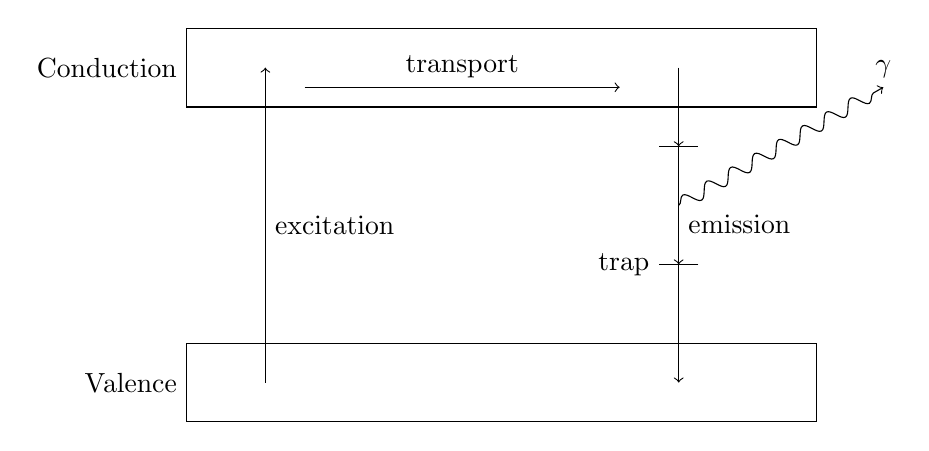
\begin{tikzpicture}[->]
		\draw (0,0) rectangle++(8,1);
		\draw (0,-3) rectangle++(8,-1);
		
		\draw (1,-3.5) -- ++(0,2) node[right] {excitation} -- ++(0,2);
		
		\draw (1.5,0.25) -- ++(2,0) node [above] {transport} -- ++(2,0);
		
		\draw[-] (6,-0.5) -- ++(0.5,0);
		\draw[-] (6.5,-2) -- ++(-0.5,0) node [left] {trap};
		
		\draw (6.25,0.5) -- ++(0,-1);
		\draw (6.25,-0.5) -- ++(0,-0.75) coordinate(emission) -- ++(0,-0.75);
		\draw (6.25,-2) -- ++(0,-1.5);
		
		\draw[decorate, decoration=snake] (emission) -- ++(30:3) node [above] {$\gamma$};
		\node[below right] at (emission) {emission};
		
		
		\node[left] at (0,0.5) {Conduction};
		\node[left] at (0,-3.5) {Valence};
	\end{tikzpicture}
	\caption{Mechanism for crystal scintillators}
	\label{fig:scintillator}
\end{figure}
Another method is to detect the muonic component, this can be done through Scintillator detectors. Due to the muon being a charged particle, it interacts with matter and deposits energy. Certain materials can give off this energy via photons, a process which is known as scintillation. Figure \ref{fig:scintillator} shows the mechanism through which scintillation occurs. First, an electron is excited from the valence band into the conduction band through energy deposit from an incident particle. This electron then is transported through the conduction band where it can drop back down to the valence band. Though if it dropped back directly, a photon would be emitted which could immediatly excit another electron in the valence band. What makes scintillators special is the existance of traps which reduce the energy of the emitted photons. Those photons then do not have enough energy to excite eletrons in the material so they can pass through it. With the use of a photmultiplier, the emitted photons can then be detected.
\section{Detector Network}
Since one detector alone only provides the timestamp of one particle hit, it does not provide useful information on its own. That is why for real measurements a network of detectors has to be used. The network on which this thesis is based consists of low-cost plastic scintillator detector units utilising a RaspberryPi minicomputer addon board as readout electronics.


The detector network is made up of a number of low-cost scintillator detectors. Each detector consists of a scintillator with \acrfull{sipm} assembly, an interface board with \acrfull{adc} and a RaspberryPi minicomputer. The interface board analyses signals from the \acrshort{sipm}, retrieves the current timestamp and passes this timestamped event along to a software running on the RaspberryPi minicomputer which sends it to a server. Each timestamped event is thus written to a central database where it can be further analysed at a later time. Due to the number of detectors and their respective rate of few Hz, a large number of events is writen to the database. This causes a large strain on the server infrastructure when running post-analysis programs since they need to handle large amounts of data in a short period of time. Since this is sub-optimal, a realtime solution which performs as much analysis and pre-filtering as possible in order to reduce the runtime impact of the analysis is preferable.

\section{Real-time analysis}
\subsection{Coincidence criteria}
A sturdy criterium to define a coincidence has to be found. Initially the criterium was defined as the $\Delta{t}$ of two events being lower than $100\,\mu\text{s}$, which corresponds to a maximum possible detector distance of $29.97\,\text{km}$. Since in reality the maximum coincidence interval is dependent on the actual detector distance and is limited by the flight distance of a muon, this criterium must be improved upon. A first approach lies in calculating the distance between the detector pair belonging to the coincidence event which is to be analysed. This is implemented as the euclidean distance derived from the detector coordinates. Therefore the WGS84 earth coordinate model has been implemented to be able to convert a given pair of geodetic coordinates to relative carthesian coordinates, specifically in the \acrfull{enu} system. The WGS84 model thereby approximates the shape of earth as an oblate spheroid. Given the straight line distance, the time of flight given the speed of light in vacuum $c_0$ can be taken as a first approximation for the expected maximum coincidence window.

This value however still needs to be refined in two ways. firstly, a minimum value has to be set due to limitations of the possible time resolution of the timestamping of each event and a not well understood per-detector timing offset on the order of magnitude of few tens of ns. This is especially critical in the case of detectors which are close together, since their calculated time of flight is only few ns, and thus would cut off a significant number of coincidence events. In order to mitigate this, a minimum coincidence window of $150\,\text{ns}$ width is defined. This value is chosen to reliably capture all coincidence events for even the closest detector pairs.

A maximum upper coincidence window width has to be defined too, though this requires a more in depth analysis. \todo{upper coincidence window}
\subsection{Coincidence and plausability determination}
In order to determine coincidences, each event needs to be checked against all other events which are currently in the event buffer.
\subsection{Resolving conflicting data}
\clearpage 
\section{Program layout}
The path of an event in the program is shown in figure \ref{fig:programlayout}. The source receives the event data and passes it on to the Station supervision class. It supervises the runtime data of each detector station and classifies it into reliability states. The specific criteria are described in the flowchart in figure \todo{make flowchart}.
\begin{figure}[ht!]
	\centering
	\begin{tikzpicture}[->]
		\node (source) [draw, process,minimum height=1cm] {Event Source};
		\node (supervision) [below=of source, draw, process,minimum height=1cm] {Station supervision};
		\node (filter) [below=of supervision, draw, process,minimum height=1cm] {Coincidence filter};
		\node (refinement) [below=of filter, draw, process,minimum height=1cm] {Coincidence refinement};
		\node (sink) [below=of refinement, draw, process,minimum height=1cm] {Event Sink};

		\node (criterium) [left=of filter, draw, process,minimum height=1cm] {Coincidence criterium};
		
		\draw (source) -- (supervision);
		\draw (supervision) -- (filter);
		\draw (filter) -- (refinement);
		\draw (refinement) -- (sink);
		
		\draw[<->] (criterium) -- (filter);
	\end{tikzpicture}
	\caption{Program layout}
	\label{fig:programlayout}
\end{figure}

\begin{figure}[ht!]
	\centering
	\begin{tikzpicture}[->]
		\node (terminal1) at (0,0) [draw, terminal] {START};
		\node (decide1) [below=of terminal1, draw, decision] {detector known};
		\node (predproc1) [below=of decide1, draw, predproc, align=left] {calculate event rates};
		\node (decide2) [below=of predproc1, draw, decision] {detector is reliable};
		\node (terminal2) [below=of decide2, draw, terminal] {pass to coincidence filter};
		\node (terminal3) [right=of predproc1, draw, terminal] {discard event};
		
		\node (decide1r) [right=of decide1] {no};
		\node (decide2r) [right=of decide2] {no};
		
		
		\draw (terminal1) -- (decide1);
		\draw (decide1) -- (predproc1);
		\draw (predproc1) -- (decide2);
		\draw (decide2) -- (terminal2);
		\draw (decide1) -- (decide1r) -| (terminal3);
		\draw (decide2) -- (decide2r) -| (terminal3);
	\end{tikzpicture}
\end{figure}
\begin{figure}[ht!]
	\centering
	\begin{tikzpicture}[->]
		\node (terminal1) at (0,0) [draw, terminal] {START};
		\node (decide1) [below=of terminal1, draw, decision] {constructor available};
		\node (predproc1) [below=of decide1, draw, predproc, align=left] {select next constructor};
		\node (decide2) [below=of predproc1, draw, decision] {criterium met};
		\node (predproc2) [below=of decide2, draw, predproc] {add event to constructor};
		\node (terminal2) [below=of predproc2, draw, terminal] {END};
		
		\node (decide1r) [right=of decide1] {no};
		\node (decide2l) [left=of decide2] {no};
		
		
		\draw (terminal1) -- (decide1);
		\draw (decide1) -- (predproc1);
		\draw (predproc1) -- (decide2);
		\draw (decide2) -- (predproc2);
		\draw (predproc2) -- (terminal2);
		\draw (decide1) -- (decide1r) |- (terminal2);
		\draw (decide2) -- (decide2l) |- (decide1);
	\end{tikzpicture}
\end{figure}
\begin{figure}[ht!]
	\centering
	\begin{tikzpicture}[->]
		\node (terminal1) at (0,0) [draw, terminal] {START};
		\node (decide1) [below=of terminal1, draw, decision] {constructor is timed out};
		\node (predproc1) [below=of decide1, draw, predproc, align=left] {select next constructor};
		\node (decide2) [below=of predproc1, draw, decision] {criterium met};
		\node (predproc2) [below=of decide2, draw, predproc] {add event to constructor};
		\node (terminal2) [below=of predproc2, draw, terminal] {END};
		
		\node (decide1r) [right=of decide1] {no};
		\node (decide2l) [left=of decide2] {no};
		
		
		\draw (terminal1) -- (decide1);
		\draw (decide1) -- (predproc1);
		\draw (predproc1) -- (decide2);
		\draw (decide2) -- (predproc2);
		\draw (predproc2) -- (terminal2);
		\draw (decide1) -- (decide1r) |- (terminal2);
		\draw (decide2) -- (decide2l) |- (decide1);
	\end{tikzpicture}
\end{figure}
\section{Primary reconstruction}
\subsection{Possible primary incident angles}
Through the assumptions shown in figure \ref{fig:angle-assumptions}, the possible source directions of a primary particle can be reduced. There, the geometry of a coincidence with $n=2$ is shown. Since she shower front can be simplified as a spherical section and the propagation speed can be assumed to be near the speed of light, two spheres with a shared tangent can be constructed. One spherical surface is the shower front, the other is a sphere around the detector which had the later event timing. Its radius $\ell$ is equal to the propagation time of light for the coincidence time. Through geometrical analysis of this arrangement, the Radius and angle pair can be derived as a function of the angle $\alpha$. This creates a curve in the plane on which the primary interaction must have taken place. Due to the symmetry of this arrangement however, in 3-D space, this curve becomes a rotational surface. \\
In the case of a coincidence with $n>2$ multiple curves can be calculated relative to the same root detector. This allows for the intersection points of each rotational surface to be calculated, which results in a reduced possible origin area for the primary interaction. \\
Given that the shower front is not a complete spherical surface but only a spherical section, the possible origin directions can be reduced with this approach. In the case of higher coincidence numbers, the possible direction can be reduced further. Additionally to the possible directions, this approach also provides a lower limit for the shower radius and footprint radius, suggesting a minimum Particle energy.
\begin{figure}[ht!]
	\centering
	\begin{tikzpicture}
		\fill (0,0) coordinate(det1) circle(0.1);
		\fill (6,0) coordinate(det2) circle(0.1);
		\draw (det2) circle(1);
		\draw (det2) -- ++(125:0.7) node[right] {$\ell$} -- ++(125:6.4) coordinate(center);
		\draw[dashed] (det2) ++(125:1) ++ (215:2) -- ++(35:4) node[right] {tangent};
		\draw (det2) ++ (125:1) arc(-55:-35:6.1) arc(-35:-125:6.1) node[left] {shower front};
		\draw (center) -- (det1) -- (det2);
		\draw (center) -- ++(0,-6.1);
		\draw[<->] (center) ++(-55:1) arc(-55:-90:1);
		\draw[<->] (center) ++(-55:1) arc(-55:-90:1);
		\draw (det2) ++(125:1) -- (det1);
		\draw (det2) ++(125:1) -- ++(0,1) -- ++(0,-2);
		
		\draw[<->] (det2) ++(125:0.25) arc(-55:-90:0.75) node[above right] {$\alpha$};
		
	\end{tikzpicture}
	\caption{Assumption for possible incidence angles}
	\label{fig:angle-assumptions}
\end{figure}
\begin{equation}
	\gamma = \frac{\pi}{2} - \alpha - \arctan\left(\frac{\ell\cdot\cos\alpha}{d - \ell\sin\alpha}\right)
\end{equation}
\begin{equation}
	\frac{\delta}{2} = \frac{\pi}{2} - \gamma = \alpha + \arctan\left(\frac{\ell\cdot\cos\alpha}{d - \ell\sin\alpha}\right)
\end{equation}
\begin{equation}
	\begin{aligned}
	\xi &= \frac{\pi}{2} - \delta - \left(\gamma + \beta\right) = \frac{\pi}{2} - 2\left(\alpha + \arctan\left(\frac{\ell\cdot\cos\alpha}{d - \ell\sin\alpha}\right)\right) - \left(\frac{\pi}{2} - \alpha\right) \\
	&= -3\alpha - 2\arctan\left(\frac{\ell\cdot\cos\alpha}{d - \ell\sin\alpha}\right)
\end{aligned}
\end{equation}
\begin{equation}
	r = \frac{s}{2\cdot\sin\left(\frac{\delta}{2}\right)}
\end{equation}
\clearpage
\section{Conclusion}
\clearpage
\backmatter
\end{document}
